\section{Theoretische Grundlagen}
\label{sec:Theorie}

Der zweite Hauptsatz der Thermodynamik besagt, dass Wärme immer vom wärmeren zum kälteren Reservoir fließt. Dieser Prozess lässt sich allerdings auch umkehren.
Es ist allerdings auch möglich, diesen Prozess umzukehren. Dies kann man realisieren mittels einer Wärmepumpe, welche dem System mechanische Arbeit zuführt. Dadurch kann dann
Wärme vom kälteren ins wärmere Reservoir transportiert wird.
.

\subsection {Güteziffer}
\label{sec:güteziffer}
Die Güteziffer $\upnu$ gibt das Verhältnis zwischen transportierter Wärmemenge und der dafür benötigten Arbeit an. Nach dem 1. Hauptsatz der Thermodynamik muss die dem Reservoir 1 hinzugefügte Wärmemenge $Q_1$
der Summe der aus Reservoir 2 entzogenen Wärmemenge $Q_2$ und der mechanischen Arbeit $A$, im vorliegenden Versuch durch die Kompressionsarbeit realisiert, sein.
Daraus ergibt sich dann für
\begin{equation}
  \upnu=\frac{Q_1}{A}
\end{equation}

\subsection {Massendurchsatz}
\label{sec:massendurchsatz}
\subsection {Berechnung der Kompressionsleistung}
\label{sec:kompressorleistung}

\subsection{Versuchsaufbau}
\label{sec:Versuchsaufbau}
%\begin{figure}
%	\centering
%	\caption{Schematische Darstellung des Versuchsaufbaus \cite{anleitung}.}
%	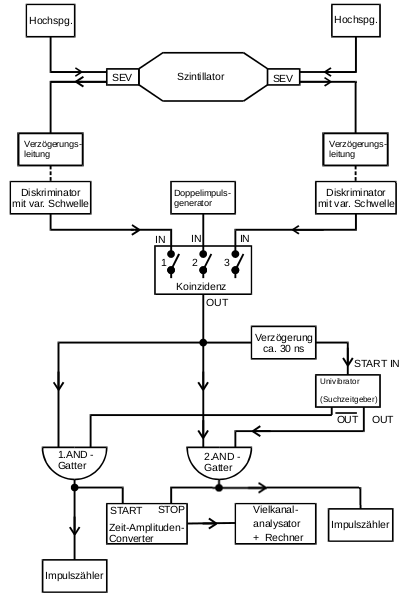
\includegraphics{Bilder/aufbau.png}
%	\label{fig:aufbau}
%\end{figure}
%
%\begin{figure}
%	\centering
%	\caption{Schematische Darstellung der Quelle zur Erzeugung radioaktiven Isotopen \cite{anleitung}.}
%	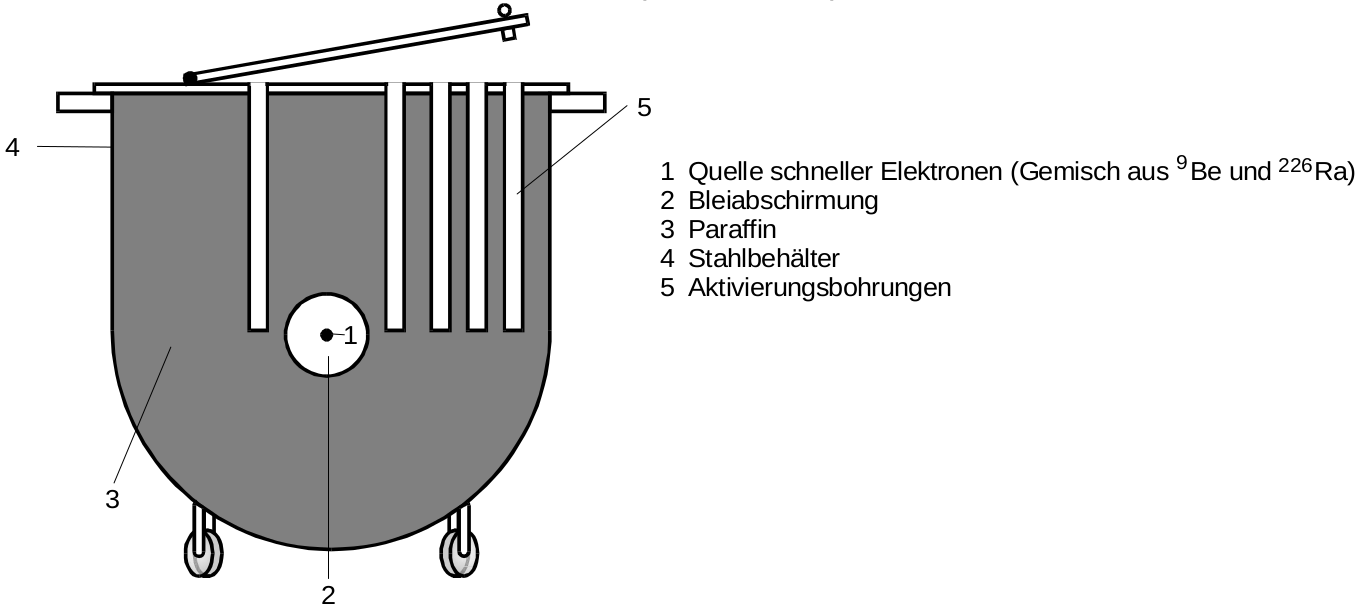
\includegraphics{content/toepfchen.png}
%	\label{fig:kochen}
%\end{figure}
%
Der Versuchsaufbau -- wie in Abbildung \ref{fig:aufbau} dargestellt -- besteht im Wesentlichen 
aus einem zerfallenden radioaktiven Isotop und einem Geiger-Müller-Zählrohr, welches die 
zerfallenden Kerne misst.
Das Geiger-Müller-Zählrohr ist entspricht einer mit Gas gefüllten Röhre. Trifft ein $\beta$-
oder $\gamma$- Teilchen auf ein Gasteilchen wird dieses ionisiert und kann aufgrund einer
anliegenden Spannung an der Röhre gemessen werden.
Dabei werden die gemessenen Zerfälle pro Messzeitintervall, welches am Zeitgeber einstellbar 
ist, an den Zählern 1 und 2 angezeigt. Nach jedem Messvorgang wird der Zähler umgeschaltet und 
der vorherige Wert auf dem aktuellen Zähler wird überschrieben. Der Versuchsaufbau ist mit
einer Blei-Abschirmung ausgestattet um die radioaktive Strahlung abzuschirmen.

Zur Erzeugung der radioaktiven Isotope wird das Objekt in Abbildung \ref{fig:kochen} verwendet.
Hierbei werden stabile Kerne mit niederenergetischen Neutronen beschossen. 
Da die Neutronen ihre Energie durch elastische Stöße an die Kerne übergeben und die maximale
Energie bei gleichen Massen der Stoßpartner erreicht wird, werden die Neutronen in einem 
Paraffinmantel gebremst, bis sie die optimale Energie besitzen.








\cite{Anleitung}
